\section{Treaps}

\begin{frame}
	\frametitle{Introduction}
	As we saw in a previous lesson, BSTs are powerful data structures that operate in $\o{\text{height of the tree}}$, which can be kept to $\o{\log(n)}$ for optimal performance. \\~\\
	
	There are \textbf{many} ways to do so, but most are complicated/long/cumbersome/error-prone.
	Treaps are however quite easy to understand and to implement.
	
	\begin{block}{Look that up if you are interested}
		B-trees (especially AA trees), Red-Black trees, AVL trees, splay trees, many others.
	\end{block}
	
\end{frame}

\begin{frame}
	\frametitle{Main idea}
	Treap = (binary search) tree + heap. Any treap node respects
	\begin{itemize}
		\item the BST property: key(left child) < key(node) < key(right child);
		\item the heap property: priority(node) > priority(child).
	\end{itemize}
	If we randomly assign the priorities, the complexity of the BST operations will be $\o{\log(n)}$. We will use $d$ in big oh notation to express the depth of the tree.
\end{frame}

\begin{frame}
	\frametitle{Implementation}
	Treaps can be implemented using rotations or using the split/merge helper functions.
	As they are equivalent, we will only discuss the split/merge strategy because it is shorter. Feel free to look up the other one on the Internet.
	\begin{itemize}
		\item $\mathrm{split} (t, X)$ separates treap $t$ into treaps $l$ and $r$ containing elements $\le X$ and $> X$ respectively.
		\item $\mathrm{merge} (l, r)$ combines treaps $l$ and $r$ into treap $t$ \textit{under the assumption that every value in $l$ is $<$ than any value in $r$}.
	\end{itemize}
\end{frame}

\begin{frame}
	\frametitle{Split}

	\begin{center}
		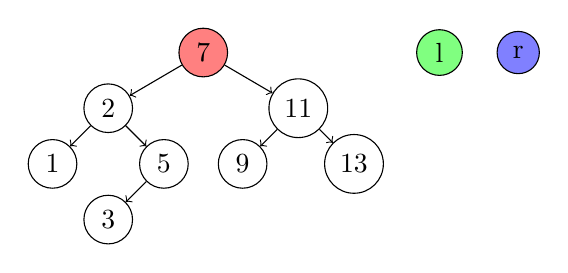
\begin{tikzpicture}[->,nodes={draw, circle}]
			\node (n0) [fill=red!50] {7};
			\node (l) [fill=green!50,xshift=3.0cm] {l};
			\node (r) [fill=blue!50,xshift=4.0cm] {r};
			\node (n1) [below left of = n0, xshift=-0.5cm]{2};
			\node (n2) [below right of = n0, xshift=0.5cm]{11};
			\node (n3) [below left of = n1]{1};
			\node (n4) [below right of = n1]{5};
			\node (n5) [below left of = n2]{9};
			\node (n6) [below right of = n2]{13};
			\node (n9) [below left of = n4]{3};
			\draw (n0) -> (n1);
			\draw (n0) -> (n2);
			\draw (n1) -> (n3);
			\draw (n1) -> (n4);
			\draw (n2) -> (n5);
			\draw (n2) -> (n6);
			\draw (n4) -> (n9);
		\end{tikzpicture}
	\end{center}
	
	Let's start with an example to understand how split works.
	We will split \col{red!50}{t} at $4$, and we will store the result in l and r. Note that priorities don't matter when splitting.
\end{frame}

\begin{frame}
	\frametitle{Split}

	\begin{center}
		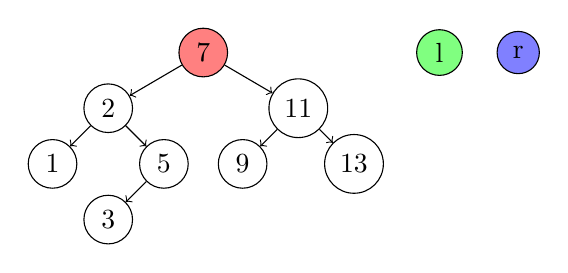
\begin{tikzpicture}[->,nodes={draw, circle}]
			\node (n0) [fill=red!50] {7};
			\node (l) [fill=green!50, xshift=3.0cm] {l};
			\node (r) [fill=blue!50, xshift=4.0cm] {r};
			\node (n1) [below left of = n0, xshift=-0.5cm]{2};
			\node (n2) [below right of = n0, xshift=0.5cm]{11};
			\node (n3) [below left of = n1]{1};
			\node (n4) [below right of = n1]{5};
			\node (n5) [below left of = n2]{9};
			\node (n6) [below right of = n2]{13};
			\node (n9) [below left of = n4]{3};
			\draw (n0) -> (n1);
			\draw (n0) -> (n2); 
			\draw (n1) -> (n3);
			\draw (n1) -> (n4);
			\draw (n2) -> (n5);
			\draw (n2) -> (n6);
			\draw (n4) -> (n9);
		\end{tikzpicture}
	\end{center}

	We see that \col{red!50}{t} has a value of 7, which is $> 4$.
	Hence \col{red!50}{t} and its right subtree clearly belong to \col{blue!50}{r}.
\end{frame}

\begin{frame}
	\frametitle{Split}

	\begin{center}
		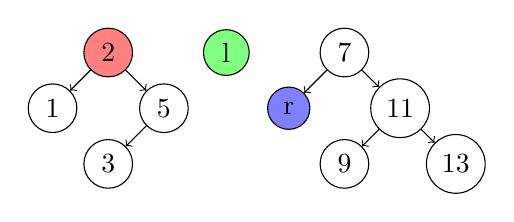
\begin{tikzpicture}[->,nodes={draw, circle}]
			\node (n0) [xshift=3.0cm] {7};
			\node (l) [fill=green!50, xshift=1.5cm] {l};
			\node (r) [fill=blue!50, below left of = n0] {r};
			\node (n1) [fill=red!50]{2};
			\node (n2) [below right of = n0]{11};
			\node (n3) [below left of = n1]{1};
			\node (n4) [below right of = n1]{5};
			\node (n5) [below left of = n2]{9};
			\node (n6) [below right of = n2]{13};
			\node (n9) [below left of = n4]{3};
			\draw (n0) -> (r);
			\draw (n0) -> (n2);
			\draw (n1) -> (n3);
			\draw (n1) -> (n4);
			\draw (n2) -> (n5);
			\draw (n2) -> (n6);
			\draw (n4) -> (n9);
		\end{tikzpicture}
	\end{center}

	We see that \col{red!50}{t} has a value of 2, which is $\le 4$.
	Hence \col{red!50}{t} and its left subtree clearly belong to \col{green!50}{l}.
\end{frame}

\begin{frame}
	\frametitle{Split}

	\begin{center}
		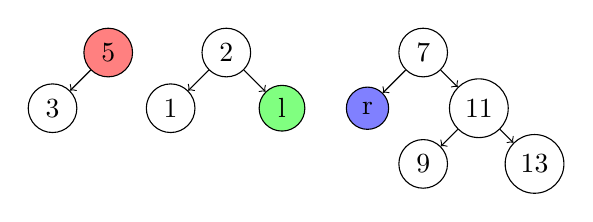
\begin{tikzpicture}[->,nodes={draw, circle}]
			\node (n0) [xshift=4.0cm] {7};
			\node (r) [fill=blue!50, below left of = n0] {r};
			\node (n1) [xshift=1.5cm] {2};
			\node (l) [fill=green!50, below right of = n1] {l};
			\node (n2) [below right of = n0]{11};
			\node (n3) [below left of = n1]{1};
			\node (n4) [fill=red!50]{5};
			\node (n5) [below left of = n2]{9};
			\node (n6) [below right of = n2]{13};
			\node (n9) [below left of = n4]{3};
			\draw (n0) -> (r);
			\draw (n0) -> (n2);
			\draw (n1) -> (n3);
			\draw (n1) -> (l);
			\draw (n2) -> (n5);
			\draw (n2) -> (n6);
			\draw (n4) -> (n9);
		\end{tikzpicture}
	\end{center}

	We see that \col{red!50}{t} has a value of 5, which is $> 4$.
	Hence \col{red!50}{t} and its right subtree clearly belong to \col{blue!50}{r}.
\end{frame}

\begin{frame}
	\frametitle{Split}

	\begin{center}
		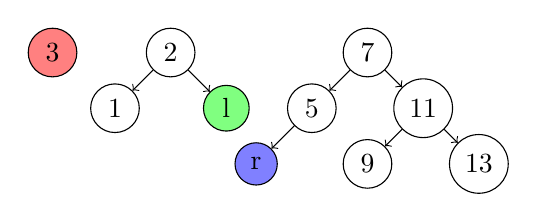
\begin{tikzpicture}[->,nodes={draw, circle}]
			\node (n0) [xshift=4.0cm] {7};
			\node (n1) [xshift=1.5cm]{2};
			\node (l) [fill=green!50, below right of = n1] {l};
			\node (n2) [below right of = n0]{11};
			\node (n3) [below left of = n1]{1};
			\node (n4) [below left of = n0]{5};
			\node (r) [fill=blue!50, below left of = n4] {r};
			\node (n5) [below left of = n2]{9};
			\node (n6) [below right of = n2]{13};
			\node (n9) [fill=red!50]{3};
			\draw (n0) -> (n4);
			\draw (n0) -> (n2);
			\draw (n1) -> (n3);
			\draw (n1) -> (l);
			\draw (n2) -> (n5);
			\draw (n2) -> (n6);
			\draw (n4) -> (r);
		\end{tikzpicture}
	\end{center}

	We see that \col{red!50}{t} has a value of 3, which is $\le 4$.
	Hence \col{red!50}{t} and its left subtree clearly belong to \col{green!50}{l}.
\end{frame}

\begin{frame}
	\frametitle{Split}

	\begin{center}
		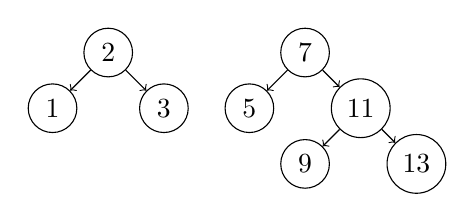
\begin{tikzpicture}[->,nodes={draw, circle}]
			\node (n0) [xshift=2.5cm] {7};
			\node (n1) []{2};
			\node (n2) [below right of = n0]{11};
			\node (n3) [below left of = n1]{1};
			\node (n4) [below left of = n0]{5};
			\node (n5) [below left of = n2]{9};
			\node (n6) [below right of = n2]{13};
			\node (n9) [below right of = n1]{3};
			\draw (n0) -> (n4);
			\draw (n0) -> (n2);
			\draw (n1) -> (n3);
			\draw (n1) -> (n9);
			\draw (n2) -> (n5);
			\draw (n2) -> (n6);
		\end{tikzpicture}
	\end{center}

	And... we are done! Implementation time!
\end{frame}

\begin{frame}
	\frametitle{Treap node}

	\lstinputlisting{src/node.cpp}

	You can obviously change key and value depending on the problem you are trying to solve.
\end{frame}

\begin{frame}
	\frametitle{Split implementation}

	\begin{center}
		\lstinputlisting{src/split_naive.cpp}
	\end{center}

	This is the straightforward implementation of the split function. It should be easy to understand. Note that we need a pointer to a pointer if we want to modify an edge (which is already a pointer by itself).
\end{frame}

\begin{frame}
	\frametitle{Split implementation}

	\begin{center}
		\lstinputlisting{src/split_pointers.cpp}
	\end{center}

	This is a compressed version of the split function.
\end{frame}

\begin{frame}
	\frametitle{Split implementation}

	\begin{center}
		\lstinputlisting{src/split.cpp}
	\end{center}

	This is the same compressed version with references instead of pointers. You should use this one in contests. \\~\\
\end{frame}

\begin{frame}
	\frametitle{Merge}

	Merge is simpler than split because less things are going on.
	Let's see how we merge \col{green!50}{l} and \col{blue!50}{r} into \col{red!50}{t}.

	\begin{center}
		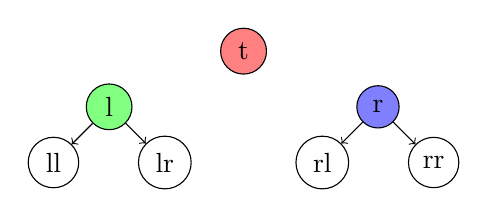
\begin{tikzpicture}[->,nodes={draw, circle}]
			\node (t) [fill=red!50] {t};
			\node (l) [fill=green!50, below left of = t, xshift = -1cm] {l};
			\node (r) [fill=blue!50, below right of = t, xshift = +1cm] {r};
			\node (ll) [below left of = l] {ll};
			\node (lr) [below right of = l] {lr};
			\node (rl) [below left of = r] {rl};
			\node (rr) [below right of = r] {rr};
			\draw (l) -> (ll);
			\draw (l) -> (lr);
			\draw (r) -> (rl);
			\draw (r) -> (rr);
		\end{tikzpicture}
	\end{center}
\end{frame}

\begin{frame}
	\frametitle{Merge}

	We can either assign \col{green!50}{l} or \col{blue!50}{r} to \col{red!50}{t} and recursively merge whatever's left.
	
	\begin{center}
		\begin{tabular}{r|l}
			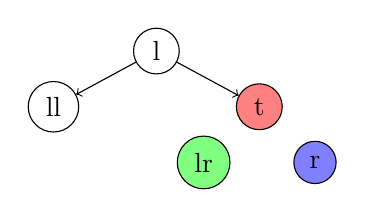
\begin{tikzpicture}[->,nodes={draw, circle}]
				\node (l) [] {l};
				\node (t) [fill=red!50, below right of = l, xshift = +0.6cm] {t};
				\node (r) [fill=blue!50, below right of = t] {r};
				\node (ll) [below left of = l, xshift = -0.6cm] {ll};
				\node (lr) [fill=green!50, below left of = t] {lr};
				\draw (l) -> (ll);
				\draw (l) -> (t);
			\end{tikzpicture}
			& 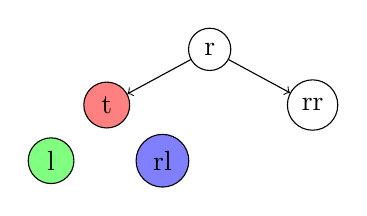
\begin{tikzpicture}[->,nodes={draw, circle}]
				\node (r) [] {r};
				\node (t) [fill=red!50, below left of = r, xshift = -0.6cm] {t};
				\node (l) [fill=green!50, below left of = t] {l};
				\node (rr) [below right of = r, xshift = +0.6cm] {rr};
				\node (rl) [fill=blue!50, below right of = t] {rl};
				\draw (r) -> (rr);
				\draw (r) -> (t);
			\end{tikzpicture}
		\end{tabular}
	\end{center}

	How do we choose? Priorities, of course! \\~\\
	Note that merge doesn't care about the keys because of the assumption that every key in l is smaller than every key in r.
\end{frame}

\begin{frame}
	\frametitle{Merge implementation}

	\begin{center}
		\lstinputlisting{src/merge.cpp}
	\end{center}
\end{frame}

\begin{frame}
	\frametitle{Insert implementation}

	To insert a node with key $X$ we assign it a random priority $P$, we go down the treap until we find a node with priority $< P$. Then we split that node at $X$ and replace it with the node.
	
	\begin{center}
		\lstinputlisting{src/insert.cpp}
	\end{center}
\end{frame}

\begin{frame}
	\frametitle{Erase implementation}

	To erase the node with key $X$, we find it and then merge its children.

	\begin{center}
		\lstinputlisting{src/erase.cpp}
	\end{center}
\end{frame}

\begin{frame}
	\frametitle{Keep track of size}

	You can lazily keep track of the size of a treap, with no additional complexity. Add a size field to the node struct and update it at the end of split, merge, insert and erase.

	\begin{center}
		\lstinputlisting{src/size.cpp}
	\end{center}
\end{frame}

\begin{frame}
	\frametitle{Additional queries}

	We can use this information to quickly find the index of the element with key $X$.

	\begin{center}
		\lstinputlisting{src/find_index.cpp}
	\end{center}
\end{frame}

\begin{frame}
	\frametitle{Additional queries}

	We can also perform range ... queries on a key interval. Here is a Range Minimum Query example:

	\begin{center}
		\lstinputlisting{src/range_min.cpp}
	\end{center}
\end{frame}

\begin{frame}
	\frametitle{Conclusion}

	Treaps are easy to implement and support a wide range of operations, all in $\o{d}$. Haven't had enough? Time to introduce you to implicit treaps.
\end{frame}

\section{Implicit treaps}

\begin{frame}
	\frametitle{Implicit treaps}

	An implicit treap is a treap that uses the index of an element as its (implicit) key, like an array. Additionally, it supports insertion/deletion/modification and all kinds of range updates and queries, just like a standard treap. \\~\\
	For this to work, we need to keep track of the position of the current element everywhere we would have used the key in a standard treap.
\end{frame}

\begin{frame}
	\frametitle{Modified split implementation}

	Here is a modified split implementation for reference. Insert and erase are left as an exercise.

	\begin{center}
		\lstinputlisting{src/implicit_split.cpp}
	\end{center}
\end{frame}

\begin{frame}
	\frametitle{Range updates}

	Treaps support range updates with lazy propagation. Just propagate at the beginning of every function. \\~\\
	Example problem: reverse interval [l, r] up to $10^5$ times. Ideas?
\end{frame}

\begin{frame}
	\frametitle{Range reverse}
	
	\begin{center}
		\lstinputlisting{src/range_reverse.cpp}
	\end{center}
\end{frame}

